
%(BEGIN_QUESTION)
% Copyright 2007, Tony R. Kuphaldt, released under the Creative Commons Attribution License (v 1.0)
% This means you may do almost anything with this work of mine, so long as you give me proper credit

Examine this process trend, showing the response of the process variable to a 10\% up-and-down step change in the controller output (placed in manual mode):

$$\includegraphics[width=15.5cm]{i01719x01.eps}$$

Something about the process variable's response should worry you, if you were tasked with tuning this process for optimum control.  Explain what is so worrisome about this trend, and identify some possible causes.

\vskip 20pt \vbox{\hrule \hbox{\strut \vrule{} {\bf Suggestions for Socratic discussion} \vrule} \hrule}

\begin{itemize}
\item{} One area of confusion for new students is whether any given trend graph reveals an {\it open-loop} test or a {\it closed-loop} test.  Explain how it is possible to discern the kind of test done on this process just by looking at the trend lines.
\item{} Explain why it is important to determine whether the trend graph reveals an {\it open-loop} test or a {\it closed-loop} test.  What difference does this determination make?
\item{} Determine at least {\it two different} potential causes for the PV trend you see here.
\item{} Based on what you see here, does the controller need to be configured for {\it direct} action or for {\it reverse} action?
\end{itemize}

\underbar{file i01719}
%(END_QUESTION)





%(BEGIN_ANSWER)

The amount of dead time is enormous, compared to the time constant and reaction rate.  Possible sources include {\it transport delay} in the process and/or valve stiction combined with insufficient air flow to the (pneumatic) actuator.

%(END_ANSWER)





%(BEGIN_NOTES)

There is no good way to tune a process like this.  The first course of action is to identify the cause of the dead time and rectify that if possible.  If the dead time cannot be eliminated or at least decreased, the controller cannot take advantage of aggressive integral action which would otherwise be quite appropriate for a fast, self-regulating process such as this.

Strategies for ``surviving'' inescapable dead time include implementing a {\it sample-and-hold} PID algorithm.  In this algorithm, the controller effectively places itself in ``manual'' mode repeatedly, for periods of time equal or greater to the dead time.  It switches back to automatic mode just long enough to ``take a peek'' at the process to see what has changed, before making another adjustment to the output and switching back to manual mode for another dead-time period.

%INDEX% Control, PID tuning: predicting PID requirements based on open-loop response

%(END_NOTES)


